\documentclass[border=5mm,tikz]{standalone}
\usepackage{tikz-cd}
\usepackage{amsmath}

\begin{document}
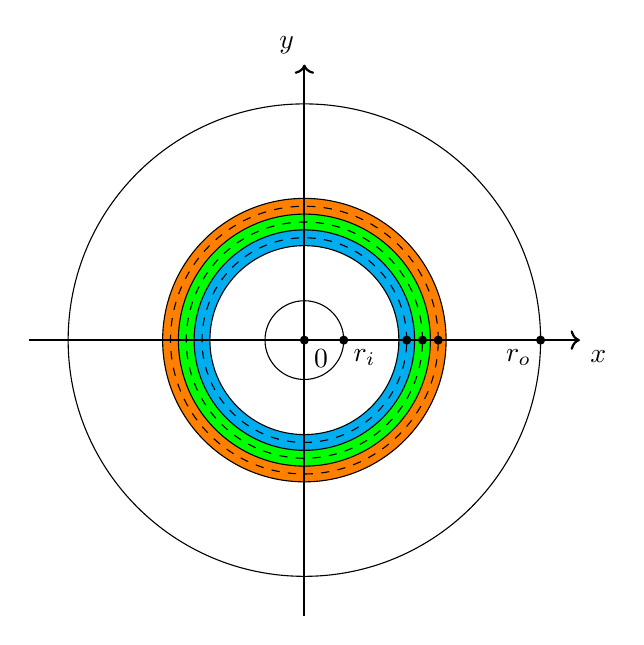
\begin{tikzpicture}

\filldraw[fill=white] (0, 0) circle [radius=3];
\filldraw[fill=orange] (0, 0) circle [radius=1.8];
\filldraw[fill=green] (0, 0) circle [radius=1.6];
\filldraw[fill=cyan] (0, 0) circle [radius=1.4];
\filldraw[fill=white] (0, 0) circle [radius=1.2];
\filldraw[fill=white] (0, 0) circle [radius=0.5];

\draw[black,dashed] (0,0) circle (1.7);
\draw[black,dashed] (0,0) circle (1.5);
\draw[black,dashed] (0,0) circle (1.3);

\draw[fill] (1.7, 0) circle [radius=0.05];
\draw[fill] (1.5, 0) circle [radius=0.05];
\draw[fill] (1.3, 0) circle [radius=0.05];

\draw[thick,->] (-3.5,0) -- (3.5,0) node[anchor=north west] {$x$};
\draw[thick,->] (0,-3.5) -- (0,3.5) node[anchor=south east] {$y$};

\draw[fill] (0,0) circle [radius=0.05];
\node [below right] at (0,0) {$0$};
\draw[fill] (3,0) circle [radius=0.05];
\node [below left] at (3,0) {$r_o$};
\draw[fill] (0.5,0) circle [radius=0.05];
\node [below right] at (0.5,0) {$r_i$};

\end{tikzpicture}
\end{document}